\documentclass[a4paper,11pt]{article}

% --- Encodage et Langue ---
\usepackage[utf8]{inputenc}
\usepackage[T1]{fontenc}
\usepackage[french]{babel}
\usepackage{slashbox}

% --- Mise en page et Typographie ---
\usepackage{geometry}
\geometry{margin=2.5cm, headheight=15pt}
\usepackage{microtype}
\usepackage{lmodern}

% --- En-têtes et pieds de page ---
\usepackage{fancyhdr}
\pagestyle{fancy}
\fancyhf{}
\renewcommand{\headrulewidth}{0pt}
\renewcommand{\footrulewidth}{0.4pt}
\fancyfoot[L]{\small\textcolor{primary}{\textit{Copyrights Jean-Christophe Le Lann -- Électronique Numérique}}}
\fancyfoot[R]{\small\textcolor{primary}{\thepage}}

% --- Mathématiques ---
\usepackage{amsmath, amssymb}
\usepackage{centernot}

% --- Images et Sous-figures ---
\usepackage{graphicx}
\usepackage{float}
\usepackage{subfig}
\usepackage{hyperref}

% --- Cartes de Karnaugh ---
\usepackage{karnaugh-map}

% --- Couleurs et Boîtes ---
\usepackage{xcolor}
\definecolor{primary}{RGB}{0, 85, 150}      % Bleu technique
\definecolor{secondary}{RGB}{240, 248, 255} % Bleu très clair pour les fonds
\definecolor{ternary}{RGB}{140, 248, 255}   % Bleu très clair pour les fonds
\definecolor{solcolor}{RGB}{245, 250, 245}  % Vert très clair pour les solutions
\definecolor{solframe}{RGB}{60, 120, 60}    % Vert foncé pour les bordures de solution

\usepackage{tcolorbox}
\tcbuselibrary{skins}
\usepackage{caption} % Pour \captionof à l'intérieur des boîtes

% --- Tableaux professionnels ---
\usepackage{booktabs}
\usepackage{array}

% --- Affichage de code / chronogrammes ---
\usepackage{listings}
\lstset{
    basicstyle=\ttfamily\small,
    backgroundcolor=\color{gray!5},
    frame=single,
    framerule=0.5pt,
    rulecolor=\color{gray!50},
    numbers=none,
    breaklines=true,
    keepspaces=true,
    columns=fullflexible
}

% --- Titres ---
\usepackage{titlesec}
\titleformat{\section}
  {\color{primary}\Large\bfseries}
  {\thesection}{1em}{}[\titlerule]
\titleformat{\subsection}
  {\color{primary}\large\bfseries}
  {\thesubsection}{1em}{}

% --- Commande personnalisée (conservée de l'original) ---
\newcommand{\op}{
\mathop{
\vphantom{\bigoplus}
\mathchoice
{\vcenter{\hbox{\resizebox{\widthof{$\displaystyle\bigoplus$}}{!}{$\boxplus$}}}}
{\vcenter{\hbox{\resizebox{\widthof{$\bigoplus$}}{!}{$\boxplus$}}}}
{\vcenter{\hbox{\resizebox{\widthof{$\scriptstyle\oplus$}}{!}{$\boxplus$}}}}
{\vcenter{\hbox{\resizebox{\widthof{$\scriptscriptstyle\oplus$}}{!}{$\boxplus$}}}}
}\displaylimits
}

% --- Gestion des solutions (Mettre \solutionsfalse pour cacher les solutions) ---
\newif\ifsolutions
\solutionstrue
%\solutionsfalse

\newtcolorbox{notebox}{
  colback=secondary,
  colframe=primary,
  fonttitle=\bfseries,
  title=Notes et Conseils,
  arc=4pt,
  boxrule=0.8pt
}

\newtcolorbox{solbox}{
  colback=solcolor,
  colframe=solframe,
  fonttitle=\bfseries,
  title=Solution,
  arc=4pt,
  boxrule=0.8pt
}


% --- Titre du document ---
\title{\textcolor{primary}{\Huge\bfseries TD 3 -- Électronique Numérique}\\[0.5em] \Large Automates ou Machines d'états finis}
\author{}
\date{}

\begin{document}

\maketitle
\thispagestyle{fancy}   % <-- AJOUTER CETTE LIGNE pour forcer le copyright sur la 1ère page
\vspace{-2em}

\begin{notebox}
\textbf{Remarque :}
Ce TD aborde plusieurs points relatifs aux \textit{automates}, aussi appelés \textit{machines d'états finis}\footnote{Ce nom quelque peu étrange signifie que le \textit{nombre} d'états est \textit{fini}. Il existe également des automates dont le nombre d'états est infini...} (\textit{finite state machines}, FSM) :
\begin{itemize}
    \item Diagrammes états-transitions : machines de Mealy et de Moore, et leur équivalence.
    \item Causalité des machines d'états finis.
    \item Conception d'un automate matériel à partir d'un diagramme états-transitions.
\end{itemize}

Les automates peuvent être vus comme l'outil conceptuel équivalent aux équations différentielles du monde analogique et continu : ces automates permettent de décrire l'évolution temporelle d'un système. Ils sont donc fondamentaux, non seulement pour la conception en Electronique, mais plus généralement pour toute l'Informatique.

\end{notebox}

% \vspace{1em}

\section{Diagramme états-transitions : Moore et Mealy}

On rappelle que le diagramme \textit{états-transitions} (ou \textit{state transition diagram}, aussi appelé \textit{diagramme à bulles}) est une représentation graphique abstraite du comportement d'un automate. Cette représentation consiste à décrire l'enchaînement des transitions d'un état à l'autre par une flèche, les états étant représentés par des cercles ou \textit{bulles}.

On distingue deux grands types de FSM
% \footnote{Attention ! Les deux automates représentés l'un à côté de l'autre ne sont pas équivalents en terme de fonctionnement. Il existe des algorithmes pour transformer Mealy en Moore (et réciproquement), de manière à obtenir des comportements identiques. Voir par exemple \url{https://fr.wikipedia.org/wiki/Machine_de_Mealy}.}
.
Dans le cas des automates de Moore, les sorties ne dépendent que des états, alors que dans le cas des automates de Mealy, les sorties dépendent à la fois des états et des entrées.

Sur les transitions, on ajoute les \textit{conditions} booléennes $c_i(s)$ qui autorisent à passer d'un état à un autre, ainsi que d'éventuelles sorties (généralement après une ou deux barres verticales) dans le cas des automates de Mealy. Lorsqu'on a affaire à un automate de Moore, les sorties sont annotées en conséquence dans les bulles (ou juste à côté).

% \begin{figure}[H]
% \centering
% \subfloat[Automate de Moore]{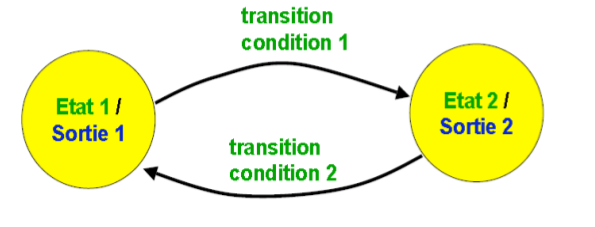
\includegraphics[width=5cm]{./images/moore.png}}
% \qquad
% \subfloat[Automate de Mealy]{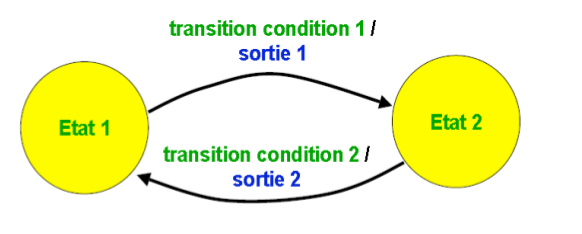
\includegraphics[width=5cm]{./images/mealy.png}}%
% \caption{FSM de Moore et Mealy}
% \label{fig:example}
% \end{figure}

\begin{figure}[H]
  \centering
  \subfloat[FSM de Moore et Mealy. Attention ! Les deux automates présentés ici ne sont ici pas équivalents en terme de comportement ! Voir exercice)]{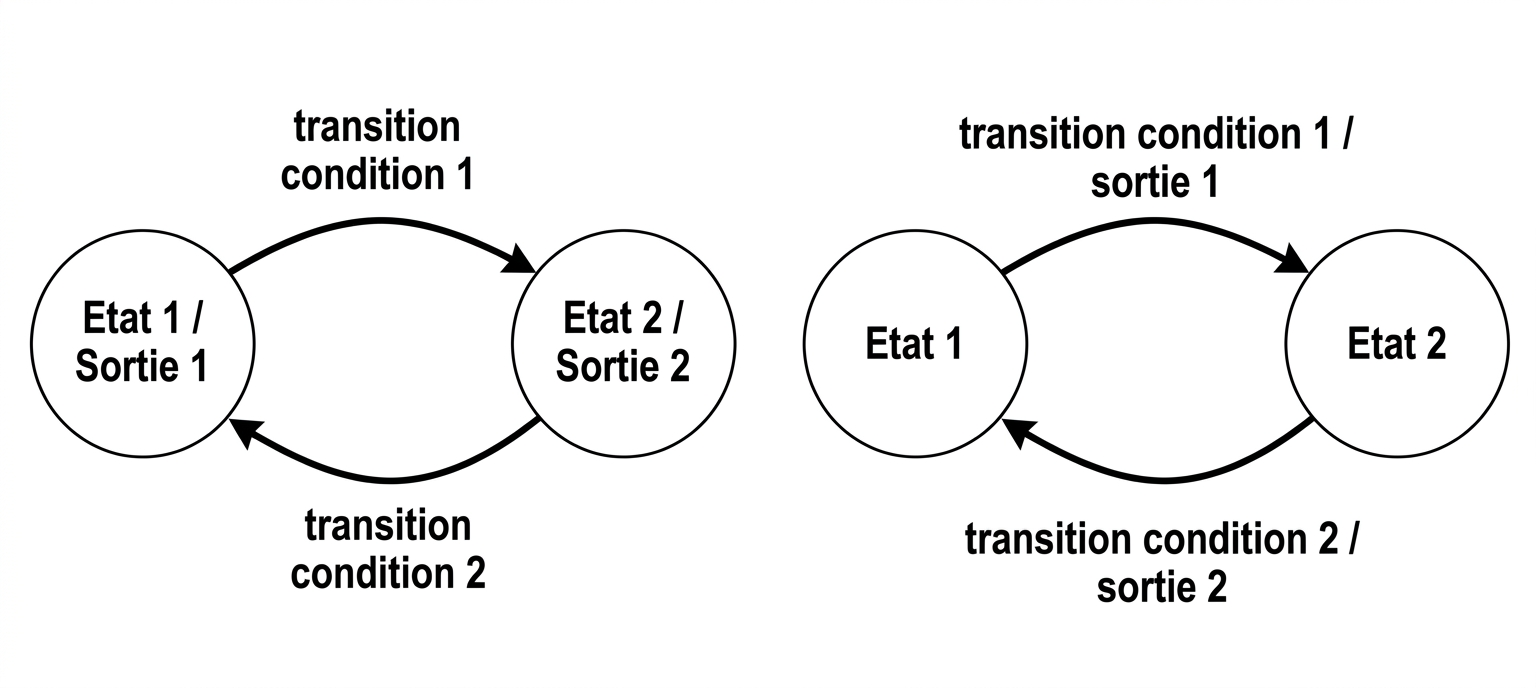
\includegraphics[width=10cm]{./images/moore_mealy.png}}
  %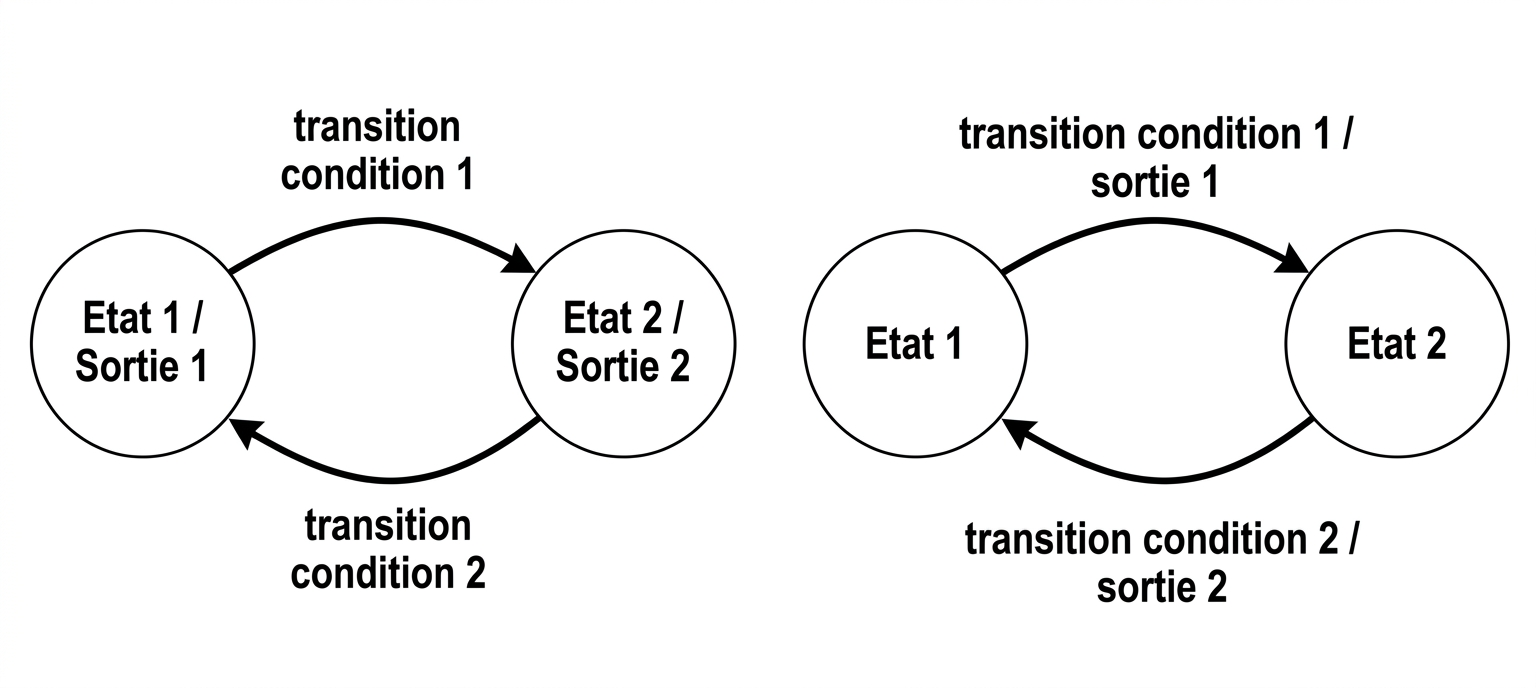
\includegraphics[width=5cm]{./images/moore_mealy.png}}
  %\caption{}
  \label{fig:example}
\end{figure}

%%\newpage
\section{Causalité d'une FSM}

Pour qu'une FSM soit considérée comme \textit{causale}, correcte ou \textit{consistante}, elle doit vérifier les deux propriétés suivantes :
\begin{itemize}
    \item \textbf{Réactivité} (exhaustivité) : il doit exister une condition vraie sur au moins une des transitions sortant d'un état.
    $$ \forall s \in S : \sum_i c_i(s)=1 $$
    \item \textbf{Déterminisme} (exclusivité) : deux conditions sur les transitions sortant d'un état ne peuvent être vraies en même temps.
    $$ \forall s \in S, \forall (i,j) \text{ avec } i \neq j, \quad c_i(s) \cdot c_j(s)=0 $$
\end{itemize}

Une autre manière de résumer ces deux propriétés est qu'il existe -- à tout instant discret -- \textit{un, et un seul, état suivant}. Notons qu'un état peut avoir comme état suivant lui-même : dans ce cas, le système décrit ne change pas d'état.

\subsection*{Questions}


\begin{enumerate}
    \item Observez la figure \ref{fig2}.Vérifier la consistance de la machine d'état suivante.
    \item Est-ce un automate de Moore ou de Mealy ?
\end{enumerate}

\begin{figure}[h] % [h] = place la figure approximativement ici
    \centering
    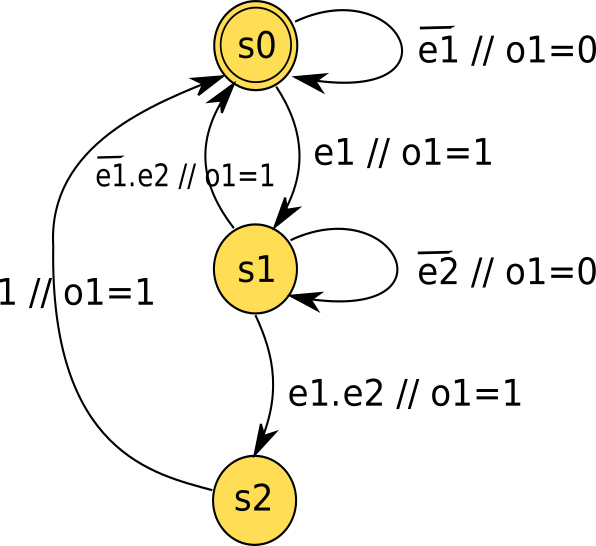
\includegraphics[scale=0.3]{./images/ex-fsm-1.png}
    \caption{FSM de l'exercice 1 et 2}
    \label{fig2}
\end{figure}

\ifsolutions
\begin{solbox}
Il y a plusieurs manières de procéder. Par exemple, on calcule les formules :
\begin{itemize}
    \item \textbf{Exhaustivité :}
    \begin{itemize}
        \item Pour S0 : $\overline{e_1} + e_1 = 1$
        \item Pour S1 : $\overline{e_2} + \overline{e_1}e_2 + e_1e_2 = 1$
        \item Pour S2 : $1 = 1$
    \end{itemize}
    \item \textbf{Exclusivité :}
    \begin{itemize}
        \item Pour S0 : $\overline{e_1} \cdot e_1 = 0$
        \item Pour S1 : $\overline{e_2}\overline{e_1}e_2 + \overline{e_2}e_1e_2 + \overline{e_1}e_2e_1e_2 = 0 + 0 + 0 = 0$
        \item Pour S2 : une seule transition. Il n'y a pas de problème d'exclusivité.
    \end{itemize}
\end{itemize}

% \vspace{0.5em}


% \vspace{0.5em}
C'est un automate de \textbf{Mealy}, car les sorties dépendent des transitions, et non pas seulement des états.
\end{solbox}
\fi

\section{Du diagramme états-transitions au circuit numérique.}
Nous cherchons ici à réaliser l'électronique de l'automate de l'exercice précédent.\\

% La méthode consiste à établir les équations logiques de la fonction \textit{état suivant}, ainsi que de la fonction (unique ici, \textit{o1}) de sortie de l'automate précédent. Ces deux ensembles nous permettront de réaliser concrètement l'électronique du circuit.\\
\begin{notebox}
  La méthode manuelle consiste à décrire tout d'abord dans un tableau :

  \begin{itemize}
    \item L'évolution des états en fonction des entrées, en conservant leur nom \textit{symbolique}.
    \item L'évolution des sorties en fonctions des états, et des entrées (cas de Mealy).
  \end{itemize}

  Après \textbf{choix d'un encodage binaire des états}, on connaît le nombre $n$ de bascules D impliquées :
\begin{itemize}
  \item On réécrit le tableau précédent pour chacune des bascules $D_i$.
  \item On déduit les équations $D_i=f(Q_0,Q_1,\dots,Q_{n-1},e_0,\dots)$, où $Q_j$ représente l'état courant de la bascule $j$ et $\{e_k\} $ l'ensemble des entrées du circuit.
\end{itemize}

\end{notebox}

 On rappelle qu'il existe un nombre infini de possibilité d'encodage des états. Cet encodage influe sur le nombre de bascules D nécessaires au stockage des états, mais également sur la complexité de la logique combinatoire de la fonction de transitions et de la fonction de sortie (et donc de la rapidité du circuit).\\

 On s'appuie sur les tableaux génériques suivants \ref{tab1} et \ref{tab2}, qui permettent de procéder de manière systématique.

 \begin{table}[htp]

   \centering
   \caption{Encodage symbolique (nom des états préservés)}\label{tab1}

   \begin{tabular}{|l|l|l|l||l|l|l|l|}
       \hline
       état courant & entrée 1 & ... & entrée n &  état suivant & sortie 1 & ... & sortie n \\ \hline
       ~        & ~    & ~         & ~            & ~            & ~        & ~   & ~        \\
       ~        & ~   & ~     & ~            & ~            & ~        & ~   & ~        \\
       \hline
   \end{tabular}

   \bigskip

   \caption{Encodage binaire (états encodés --ici sur 2 bits)}\label{tab2}

   \begin{tabular}{|l|l|l|l||l|l|l|l|l|l|}
     \hline
     Q1 & Q0 &  entrée 1 & ... & entrée n & D1 & D0 & sortie 1 & ... & sortie n \\ \hline
     ~        & ~  & ~  & ~  & ~  & ~  & ~  & ~        & ~   & ~        \\
     ~        & ~  & ~  & ~  & ~  & ~  & ~  & ~        & ~   & ~        \\
     \hline
   \end{tabular}

 \end{table}


\subsection*{Questions}
\begin{itemize}
  \item Etablir le tableau d'évolution des états symboliques et de la sortie.
  \item Choisir l'encodage \textit{dense} le plus naturel.
  \item Etablir le tableau d'évolution des états encodés et de la sortie.
  \item Etablir les équations de chacun des bits d'états.
  \item Etablir les équations de chacun des bits de sortie.
  \item Dessiner le circuit à l'aide portes logiques élémentaires.
\end{itemize}


\ifsolutions
\begin{solbox}
\renewcommand{\arraystretch}{1.2}
\begin{table}[H]
\centering
\begin{tabular}{c c c c c}
\toprule
\textbf{État courant} & $e_1$ & $e_2$ & \textbf{État suivant} & $o_1$ \\
\midrule
S0 & 0 & X & S0 & 0 \\
S0 & 1 & X & S1 & 1 \\
S1 & X & 0 & S1 & 0 \\
S1 & 0 & 1 & S0 & 1 \\
S1 & 1 & 1 & S2 & 1 \\
S2 & X & X & S0 & 1 \\
\bottomrule
\end{tabular}
\end{table}

Puis encodons les états symboliques S0, S1 et S2 par 00, 01, 10 :

\begin{table}[H]
\centering
\begin{tabular}{c c c c c c c}
\toprule
$Q_1$ & $Q_0$ & $e_1$ & $e_2$ & $D_1$ & $D_0$ & $o_1$ \\
\midrule
0 & 0 & 0 & X & 0 & 0 & 0 \\
0 & 0 & 1 & X & 0 & 1 & 1 \\
0 & 1 & X & 0 & 0 & 1 & 0 \\
0 & 1 & 0 & 1 & 0 & 0 & 1 \\
0 & 1 & 1 & 1 & 1 & 0 & 1 \\
1 & 0 & X & X & 0 & 0 & 1 \\
\bottomrule
\end{tabular}
\end{table}

\textit{Attention :} ne pas chercher les équations directement à partir de ce tableau ! Il manque des combinaisons. Utilisons plutôt le tableau de Karnaugh réorganisé :

\begin{table}[H]
\centering
\renewcommand{\arraystretch}{1.2}
\begin{tabular}{c|c c c c}
\toprule
& $\overline{e_1}\overline{e_2}$ & $\overline{e_1}e_2$ & $e_1e_2$ & $e_1\overline{e_2}$ \\
\midrule
$\overline{Q_1}\overline{Q_0}$ & 00 & 00 & 01 & 01 \\
$\overline{Q_1}Q_0$ & 01 & 00 & 10 & 01 \\
$Q_1Q_0$ & xx & xx & xx & xx \\
$Q_1\overline{Q_0}$ & 00 & 00 & 00 & 00 \\
\bottomrule
\end{tabular}
\end{table}

À partir de ce dernier tableau, on peut déterminer les équations de $D_1$, $D_0$ et $o_1$ :
\begin{align*}
    D_1 &= Q_0 \cdot e_1 \cdot e_2 \\
    D_0 &= \overline{Q_1}\overline{Q_0}e_1 + Q_0\overline{e_2} \\
    o_1 &= \overline{Q_1}\overline{Q_0}e_1 + Q_0e_2 + Q_1
\end{align*}
\end{solbox}
\fi


\section{Automate \textit{détecteur de séquence}}

Il est fréquent de devoir détecter une séquence particulière dans un flux de données. Les automates se prêtent très bien à ce genre de détection. On peut citer :
\begin{itemize}
    \item L'analyse de paquets réseaux, détection de paquets interdits (entrants ou sortants) dont on connaît une certaine signature numérique (travail de filtrage d'un proxy, etc.).
    \item L'analyse de flux multimédia : par exemple \textit{start codes} de séquences, dans un film (stocké en numérique, dans un format de compression).
    \item L'analyse génomique : il existe des accélérateurs FPGA dédiés à la reconnaissance de séquence du génome, etc.
\end{itemize}

\subsection{Détecteur de séquence \texttt{10} : Moore versus Mealy}
Dans le cadre de la conception d'un sous-système de communication série, on souhaite réaliser un détecteur de séquence capable de repérer le motif binaire \textbf{"10"} sur un flux de données synchronisé par une horloge.

Le système possède :
\begin{itemize}
    \item Une entrée binaire synchrone $X$ (le bit courant),
    \item Une sortie binaire synchrone $Z$ qui vaut \textbf{1} si et seulement si la séquence \textbf{"10"} vient d'être détectée sur l'entrée $X$, et \textbf{0} sinon.
\end{itemize}

On considère que les séquences peuvent se chevaucher (par exemple, dans la séquence \texttt{1\,1\,0}, le motif \textbf{"10"} est détecté sur les deux derniers bits).

% \subsection*{Questions}

\begin{enumerate}
    \item \textbf{Automate de Mealy.} Concevoir un automate de type \textbf{Mealy} réalisant cette fonction. On donnera :
    \begin{itemize}
        \item la description des états et leur signification,
        \item la table des transitions (format : \textit{état suivant / sortie}).
    \end{itemize}

    \item \textbf{Automate de Moore.} Concevoir un automate de type \textbf{Moore} ayant un comportement fonctionnel équivalent. On donnera :
    \begin{itemize}
        \item la description des états, leur signification et la sortie associée,
        \item la table des transitions.
    \end{itemize}

    \item \textbf{Comparaison temporelle.} Relever les valeurs de la sortie $Z$ pour les deux automates sur la séquence d'entrée suivante, appliquée à chaque front montant de l'horloge :
    \[
        X = 0,\; 1,\; 0,\; 0,\; 1,\; 1,\; 0
    \]
    On supposera que les deux automates sont initialisés dans leur état de départ avant le premier front.

    \item \textbf{Analyse.} Les deux automates sont-ils strictement équivalents ? Justifier en précisant la différence fondamentale entre les machines de Moore et de Mealy, et expliquer le phénomène observé à la question 3.
\end{enumerate}

% =====================================================================
% SOLUTION
% =====================================================================
\ifsolutions
\begin{solbox}

\textbf{1. Automate de Mealy.}

Dans un automate de Mealy, la sortie dépend de l'état \emph{présent} et de l'entrée \emph{présente}. La réaction est donc immédiate (combinatoire).

\begin{itemize}
    \item $S_0$ : état initial (aucun \texttt{1} en attente, ou dernier bit reçu = \texttt{0}).
    \item $S_1$ : on vient de recevoir un \texttt{1} (le \texttt{0} suivant complètera le motif).
\end{itemize}

\medskip
\noindent
\begin{tabular}{|c|c|c|}
\hline
\textbf{État présent} & \textbf{Si $X = 0$} & \textbf{Si $X = 1$} \\
\hline
$\rightarrow S_0$ & $S_0 \;/\; Z=0$ & $S_1 \;/\; Z=0$ \\
\hline
$S_1$             & $S_0 \;/\; \mathbf{Z=1}$ & $S_1 \;/\; Z=0$ \\
\hline
\end{tabular}

\medskip
\textbf{2. Automate de Moore.}

Dans un automate de Moore, la sortie ne dépend \emph{que} de l'état présent. Il faut donc un état supplémentaire pour \og mémoriser \fg{} le fait d'avoir détecté la séquence.

\begin{itemize}
    \item $S_0$ : état initial, sortie $Z=0$.
    \item $S_1$ : on vient de recevoir un \texttt{1}, sortie $Z=0$.
    \item $S_2$ : on vient de détecter \textbf{"10"}, sortie $\mathbf{Z=1}$.
\end{itemize}

\medskip
\noindent
\begin{tabular}{|c|c|c|c|}
\hline
\textbf{État présent} & \textbf{Sortie $Z$} & \textbf{Si $X = 0$} & \textbf{Si $X = 1$} \\
\hline
$\rightarrow S_0$ & 0 & $S_0$ & $S_1$ \\
\hline
$S_1$             & 0 & $S_2$ & $S_1$ \\
\hline
$S_2$             & 1 & $S_0$ & $S_1$ \\
\hline
\end{tabular}

\medskip
\textbf{3. Comparaison temporelle.}

Séquence d'entrée : $X = 0,\; 1,\; 0,\; 0,\; 1,\; 1,\; 0$.

\medskip
\noindent
\begin{tabular}{|c|c|c|c|c|c|c|c|}
\hline
Cycle         & 1 & 2 & 3 & 4 & 5 & 6 & 7 \\
\hline
Entrée $X$    & 0 & 1 & 0 & 0 & 1 & 1 & 0 \\
\hline
Sortie Mealy $Z$  & 0 & 0 & \textbf{1} & 0 & 0 & 0 & \textbf{1} \\
\hline
Sortie Moore $Z$  & 0 & 0 & 0 & \textbf{1} & 0 & 0 & 0 \\
\hline
\end{tabular}

\medskip
\textbf{4. Analyse.}

Les deux automates sont \textbf{fonctionnellement équivalents} : ils reconnaissent exactement la même séquence. Cependant, ils ne sont \textbf{pas synchrones temporellement}.

\begin{itemize}
    \item Dans l'automate de \textbf{Mealy}, la sortie est produite par un réseau combinatoire : dès que l'entrée $X$ passe à \texttt{0} au cycle 3 (complétant le motif \texttt{10}), la sortie $Z$ réagit \emph{immédiatement} dans le même cycle.
    \item Dans l'automate de \textbf{Moore}, la transition vers l'état $S_2$ n'est effective qu'au front d'horloge suivant. La sortie $Z=1$ n'apparaît donc qu'au cycle 4.
\end{itemize}

\medskip
\noindent
\textbf{Conclusion :} la sortie d'un automate de Moore est \textbf{toujours décalée d'un cycle d'horloge} par rapport à celle d'un automate de Mealy équivalent. En conception numérique (FPGA, ASIC), on ajoute généralement une bascule de sortie à l'automate de Mealy pour synchroniser sa sortie sur l'horloge : on élimine ainsi les rebonds combinatoires (\emph{glitches}) et on retrouve un comportement temporel identique à celui de Moore, au prix d'un cycle de latence supplémentaire.

\end{solbox}
\fi

\subsection{Détecteur de séquence \texttt{0110}}

On considère le détecteur de séquence de la figure \ref{exo2}. Son rôle est de détecter les séquences \textit{0-1-1-0} sur son unique entrée $x$. Lorsque cette séquence est détectée, il émet un \textit{1} sur sa sortie $y$. Un chronogramme est fourni à titre d'exemple. Notez que dans le flux \textit{0-1-1-0-1-1-0}, la séquence apparaît deux fois !
\begin{figure}[H]
  \centering
  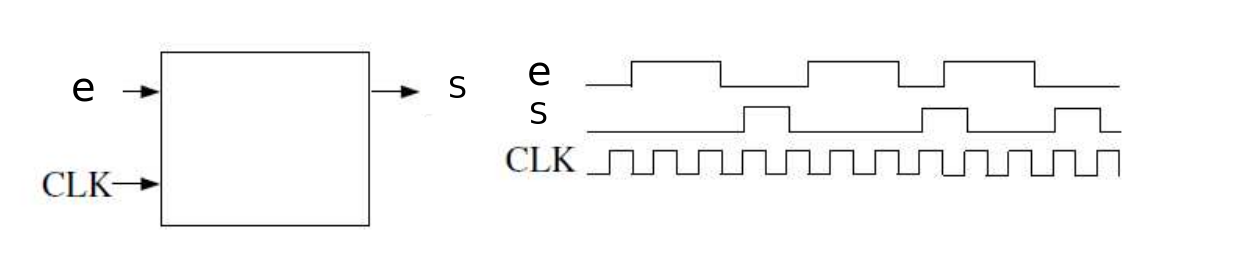
\includegraphics[scale=0.3]{./images/exo2}
  \caption{Schéma de principe du détecteur de séquence \texttt{0110}. Chronogramme associé.}
  \label{exo2}
\end{figure}

\begin{enumerate}
    \item Proposer un diagramme états-transitions pour ce détecteur. On choisira une machine de Moore.
    \item Proposer un encodage dense des états.
    \item Réaliser le circuit.
\end{enumerate}

\ifsolutions
\begin{solbox}
\centering
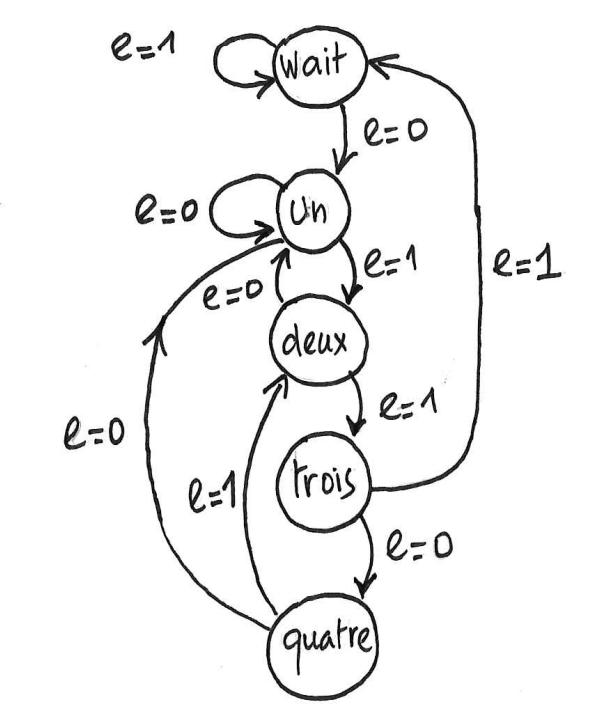
\includegraphics[scale=0.3]{./images/fsm_detect}
\captionof{figure}{Diagramme états-transitions pour le détecteur de séquences.}
\label{fsm_detect}

\vspace{0.5em}
L'automate solution est décrit sur la figure \ref{fsm_detect}. On choisit l'encodage dense suivant :

\begin{center}
\renewcommand{\arraystretch}{1.2}
\begin{tabular}{c c}
\toprule
\textbf{État} & \textbf{Code} \\
\midrule
wait & 000 \\
un & 001 \\
deux & 010 \\
trois & 011 \\
quatre & 100 \\
\bottomrule
\end{tabular}
\end{center}

On a alors la table de séquencement suivante :

\begin{center}
\renewcommand{\arraystretch}{1.2}
\begin{tabular}{|c c c c ||c c c c|}
\toprule
$Q_2$ & $Q_1$ & $Q_0$ & $e$ & $D_2$ & $D_1$ & $D_0$ & $s$ \\
\midrule
0 & 0 & 0 & 0 & 0 & 0 & 1 & 0 \\
0 & 0 & 0 & 1 & 0 & 0 & 0 & 0 \\
0 & 0 & 1 & 0 & 0 & 0 & 1 & 0 \\
0 & 0 & 1 & 1 & 0 & 1 & 0 & 0 \\
0 & 1 & 0 & 0 & 0 & 0 & 1 & 0 \\
0 & 1 & 0 & 1 & 0 & 1 & 1 & 0 \\
0 & 1 & 1 & 0 & 1 & 0 & 0 & 1 \\
0 & 1 & 1 & 1 & 0 & 0 & 0 & 0 \\
1 & 0 & 0 & 0 & 0 & 0 & 1 & 0 \\
1 & 0 & 0 & 1 & 0 & 1 & 0 & 0 \\
\bottomrule
\end{tabular}
\end{center}
\end{solbox}
\fi

\ifsolutions
\begin{solbox}
Cherchons maintenant les équations, en passant par des tableaux de Karnaugh.

\vspace{1em}
\begin{karnaugh-map}[4][4][1][$Q_2Q_1$][$Q_0E$]
   \minterms{0,1,2,5,8}
   \maxterms{4,6,9,12,13}
   \terms{3,7,10,11,14,15}{X}
   \implicant{1}{7}
   \implicantcorner
\end{karnaugh-map}
On obtient la formule : $D_0 = Q_1\overline{Q_0} + \overline{Q_1}\overline{E}$

\vspace{1em}
\begin{karnaugh-map}[4][4][1][$Q_2Q_1$][$Q_0E$]
   \minterms{5,6,8,12}
   \maxterms{0,1,2,4,9,12,13}
   \terms{3,7,10,11,14,15}{X}
   \implicant{5}{7}
   \implicant{7}{14}
   \implicantedge{12}{12}{14}{14}
\end{karnaugh-map}
On obtient la formule : $D_1 = Q_1\overline{Q_0}E + \overline{Q_1}Q_0E + Q_2E$
\end{solbox}
\fi

\ifsolutions
\begin{solbox}
\vspace{1em}
\begin{karnaugh-map}[4][4][1][$Q_2Q_1$][$Q_0E$]
   \minterms{9}
   \maxterms{0,1,2,4,5,6,8,12,13}
   \terms{3,7,10,11,14,15}{X}
   \implicant{9}{11}
\end{karnaugh-map}
On obtient la formule : $D_2 = Q_1Q_0\overline{E}$

\vspace{1em}
\begin{karnaugh-map}[4][4][1][$Q_2Q_1$][$Q_0E$]
   \minterms{2,6}
   \maxterms{0,1,4,5,8,9,12,13}
   \terms{3,7,10,11,14,15}{X}
   \implicant{3}{10}
\end{karnaugh-map}
On obtient la formule : $S = Q_2$ \textit{(Note : l'original indiquait $D_3$, mais il s'agit de la sortie $S$ ou $y$)}.
\end{solbox}
\fi

\section{Arbitre à priorité tournante (round-robin)}
% On rappelle que le diagramme à bulle est une représentation, qui se veut intuitive, du comportement séquentiel d'un automate d'états finis (FSM) : chaque état est représenté par un cercle
% (bulle) duquel peuvent partir différentes transitions (ou arcs) vers d'autres états possibles. Les transitions sont étiquetées par la condition booléenne amenant à l'état suivant.\\

On désire réaliser un circuit d'arbitrage entre deux clients susceptibles d'utiliser une ressource qui n'admet qu'un seul occupant à la fois (par exemple deux enfants qui veulent jouer au vélo,
et il n'y a qu'un vélo. Le cas se présente également dans les ordinateurs, où différents périphériques peuvent vouloir accéder à un ensemble de fils --bus central-- en même temps).
Le but du circuit est d'accorder correctement la ressource à un seul client à la fois.\\

Les clients manifestent respectivement sur $e_1$ et $e_2$ leurs désirs d'utiliser la ressource : $e_i=1$ si le client $i$ désire la ressource, $e_i=0$ s'il ne la désire pas.\\

\begin{figure}[!h]
\begin{center}
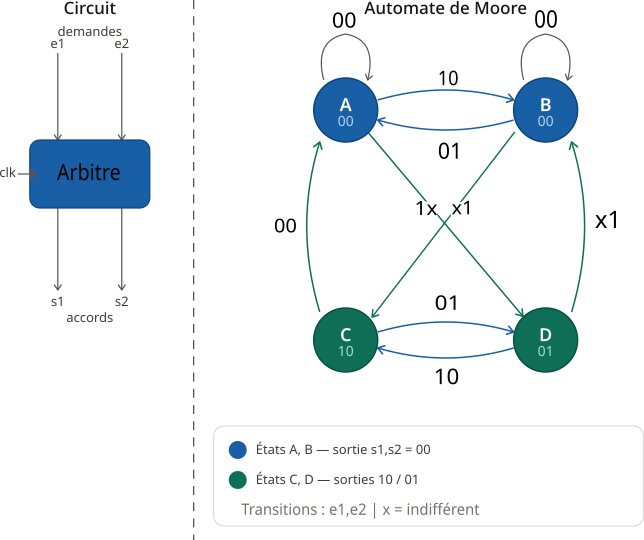
\includegraphics[scale=0.65]{./images/round_robin.png}
\end{center}
\end{figure}

Le circuit génère sur $s_1$ et $s_2$ l'attribution de la ressource à chaque client : $s_i=1$ si la ressource est attribuée au client $i$, $s_i=0$ sinon.\\

Lorsque la ressource est attribuée à un client, elle le demeure tant que le client la désire.\\

Lorsque la ressource est libre, elle est attribuée au premier qui la demande ; en cas de demandes simultanées, elle est attribuée selon une certaine priorité, mais pour éviter les injustices, la priorité entre les clients change à chaque attribution : le client qui obtient la ressource devient le moins prioriatire.\\

L'analyse du problème conduit à l'automate suivant : il y a quatre états, deux états A et B dans lesquels la ressource est libre, et deux états C et D dans lesquels la ressource est occupée.

\subsection*{Questions}
\begin{enumerate}
\item Proposer un encodage des états tel que chaque état soit codé sur 2 bits
\item Etablir la fonction de transition du système sous forme de table de vérité. Simplifier.
\item Etablir la fonction de sortie du système. Simplifier.
\item Dessiner le circuit correspondant. Combien de portes faut-il ?
\end{enumerate}

%%\newpage
\ifsolutions
\begin{solbox}
%On propose l'encodage des états a priori le plus intuitif : $A\rightarrow 00$, $B \rightarrow 01$, $C \rightarrow 10$, $D \rightarrow 11$ etc...
Cet encodage nous indique qu'il faut 2 bascules D pour stocker l'état du système. Nommons par exemple ces deux bascules $Q_1$ et $Q_0$.


  \begin{center}
        \begin{tabular}{|c||c|c|cc|}
            \hline
            Etat  & Encodage entier & Encodage binaire & $Q_1$ & $Q_0$ \\ \hline \hline
            A     & 0 & 00 & 0 & 0 \\ \hline
            B     & 1 & 01 & 0 & 1 \\ \hline
            C     & 2 & 10 & 1 & 0 \\ \hline
            D     & 3 & 11 & 1 & 1 \\ \hline
        \end{tabular}
  \end{center}


Ecrivons la table qui décrit l'évolution des entrées des bascules en fonction des entrées et de l'état courant. Dans le tableau, on a rappelé les états symboliques.


\begin{center}
      \begin{tabular}{|c|c|c|c|c||c|c|c|}
          \hline
          \multicolumn{3}{|c|}{Etat courant} & \multicolumn{2}{c||}{Entrées} & \multicolumn{3}{c|}{Etat futur} \\ \hline
          symbole  & $Q_1$ & $Q_0$ & $e_1$ & $e_2$ & $D_1$ & $D_0$ & symbole  \\ \hline \hline
          A & 0 & 0 & 0 & 0 & 0 & 0  & A \\ \hline
          A & 0 & 0 & 0 & 1 & 1 & 1 & D  \\ \hline
          A & 0 & 0 & 1 & 0 & 1 & 0 & C\\ \hline
          A & 0 & 0 & 1 & 1 & 1 & 0 & C\\ \hline \hline
          B & 0 & 1 & 0 & 0 & 0 & 1  & B\\ \hline
          B & 0 & 1 & 0 & 1 & 1 & 1  & D\\ \hline
          B & 0 & 1 & 1 & 0 & 1 & 0  & C\\ \hline
          B & 0 & 1 & 1 & 1 & 1 & 1  & D\\ \hline \hline
          C & 1 & 0 & 0 & 0 & 0 & 1  & B\\ \hline
          C & 1 & 0 & 0 & 1 & 1 & 1  & D\\ \hline
          C & 1 & 0 & 1 & 0 & 1 & 0  & C\\ \hline
          C & 1 & 0 & 1 & 1 & 1 & 0  & C\\ \hline \hline
          D & 1 & 1 & 0 & 0 & 0 & 0  & A\\ \hline
          D & 1 & 1 & 0 & 1 & 1 & 1  & D\\ \hline
          D & 1 & 1 & 1 & 0 & 1 & 0  & C\\ \hline
          D & 1 & 1 & 1 & 1 & 1 & 1  & D\\ \hline
      \end{tabular}
\end{center}

partir de ce tableau, on cherche les équations de $D_1$ et $D_0$. $D_1$ se trouve facilement, par une observation attentive du tableau : on peut voir une factorisation aisée :
$$D_1=e_1+e_2$$
\end{solbox}

%\ifsolutions
\begin{solbox}

Pour $D_0$, passons par un tableau de Karnaugh.


   \begin{center}
      \begin{tabular}{|c|c|c|c|c|}
        \hline
                \backslashbox{$Q_1.Q_0$}{$e_1.e_2$}  & 00 & 01 & 11 & 10 \\ \hline
                                                 00 &  ~ &  1 &  ~ & ~ \\
                                                 00 &  1 &  1 &  1 & ~ \\
                                                 01 &  ~ &  1 &  1 & ~ \\
                                                 11 &  1 &  1 &  ~ & ~ \\ \hline
      \end{tabular}
   \end{center}

Les regroupements amènent à :
$$D_0=\overline{e_1}.e_2+e_2.Q_0+\overline{e_1}.\overline{Q_1}.Q_0+Q_1.\overline{Q_0}.\overline{e_1}$$

Calculons les sorties, de la même manière. On trouve : $S_1=Q_1.\overline{Q_0}$ et $S_2=Q_1.Q_0$

On peut désormais dessiner le circuit complet :


\begin{center}
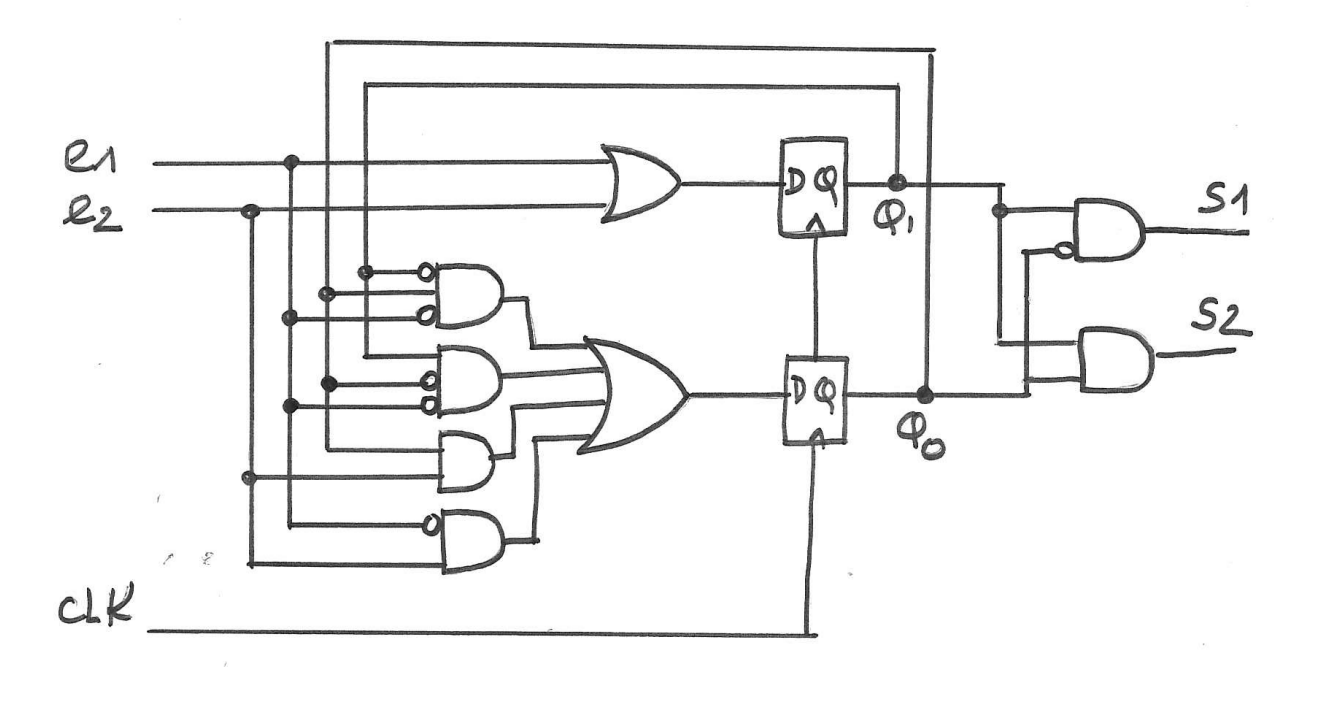
\includegraphics[scale=0.3]{./images/circuit-4.png}
\end{center}

\end{solbox}
\fi

%=======================================================================================
%                                 Dé numérique
%=======================================================================================
\section{Problème du dé électronique. Encodage des états spécifique.}

On doit réaliser une boîte équipée d'un bouton poussoir, de 7 diodes lumineuses (LEDs) d'un circuit logique (à définir) et d'une pile. Ce dispositif doit simuler un dé, lancé aléatoirement : il affiche entre 1 et 6.\\

\begin{figure}[!h]
\begin{center}
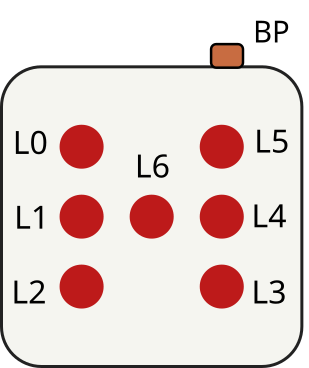
\includegraphics[scale=0.3]{./images/de.png}
\end{center}
\end{figure}

Chaque fois que l'utilisateur appuie sur le bouton-poussoir toutes les leds s'allument puis, dès que l'opérateur relâche le bouton, les LEDs se fixent sur l'une des configurations ci-dessous.\\

A l'appui sur le bouton-poussoir toutes les configurations sont affichées en séquence à la cadence d'une horloge rapide. L'utilisateur ne peut pas distinguer les combinaisons, du fait de la persistence rétinienne. Seule une illumination moyenne lui apparait.\\

On choisit d'utiliser un encodage des états particulier, \textit{spécifique au problème} : la sortie de chaque bascule $Q_i, i\in {0..6}$ pilote directement la led $L_i$ correspondante. La fonction de sortie de l'automate est ainsi la \textit{fonction identité}.

\subsection*{Question}
\begin{enumerate}
\item Réaliser le tableau décrivant l'évolution de chaque bascule lorsque le dé est sollicité (bouton poussoir appuyé).
\item En déduire les équations constitutives du circuit correspondant.
\item Dessiner le circuit d'une ou deux de ces équations.
\item Rappeler succintement le schéma-blocs composé de 2 blocs : la logique d'état suivant et les bascules D (registres).
\item Choisir un autre encodage (par exemple one-hot) et réaliser à nouveau le circuit.
\end{enumerate}



\section{La magie de l'encodage "\textit{one-hot}" ou "\textit{un bit par état}"}

Une machine distribue des canettes à 1€. Elle n'accepte que des pièces de 0,50€ et de 1€. Elle ne rend pas la monnaie.\\

On précise quelques éléments :
\begin{itemize}
    \item \textbf{Entrées :} `P50` (pièce de 50c) et `P100` (pièce de 1€). Les deux entrées ne sont jamais actives en même temps.
    \item \textbf{Sorties :} `DIST` (Distribuer la canette) et `REND` (Rendre 0,50€ de monnaie - uniquement si le client a donné 1,50€).
    \item \textbf{Fonctionnement :}
    \begin{itemize}
        \item Si somme totale atteint \textbf{1,00€} $\rightarrow$ `DIST=1`.
        \item Si somme totale atteint \textbf{1,50€} $\rightarrow$ `DIST=1` ET `REND=1` (car il a donné 1,50€ pour une canette à 1€).
    \end{itemize}
\end{itemize}

\vspace{0.5cm}
\subsection*{Questions}

\begin{enumerate}
  \item Déssiner le diagramme états-transitions en conservant le nom des états symboliques.
  \item Réaliser l'encodage \textit{one-hot}.
  \item Etablir les équations $D_i$ de chacune des bascules mises en jeu.
\end{enumerate}

% --- DÉBUT DE LA SOLUTION ---
\ifsolutions
\begin{solbox}

\subsection*{Question 1 : Définition des états}

\textbf{États possibles (somme encaissée) :}
\begin{itemize}
    \item `S0` : 0,00€ (état initial)
    \item `S50` : 0,50€
    \item `S100` : 1,00€ (on distribue puis on revient à S0)
    \item `S150` : 1,50€ (on distribue, on rend 0,50€, puis on revient à S0)
\end{itemize}

Voici l'ensemble des équations pour les entrées des 4 bascules :

\[
\begin{array}{rcl}
D_0 & = & Q_2 \; + \; Q_3 \quad \text{(retour à zéro après distribution)} \\
D_1 & = & Q_0 \cdot P50 \\
D_2 & = & Q_0 \cdot P100 \; + \; Q_1 \cdot P50 \\
D_3 & = & Q_1 \cdot P100 \; + \; Q_2 \cdot P50
\end{array}
\]

\noindent \textbf{Remarque :} En codage binaire classique, ces équations auraient nécessité des décodeurs complexes. Ici, la logique se limite à des portes ET et OU, ce qui rend la machine plus rapide et plus facile à maintenir.

\end{solbox}
\fi
% --- FIN DE LA SOLUTION ---

%=======================================================================================
%                                serrure numérique
%=======================================================================================
\section{Automate \textit{serrure numérique}. Le problème des \textit{spécifications}.}

L'accès à un local est protégé par une serrure codée associée à un automatisme commandant la gâche électrique de la porte. La combinaison secrète est : \textbf{A, D, C}.

\begin{figure}[H]
\centering
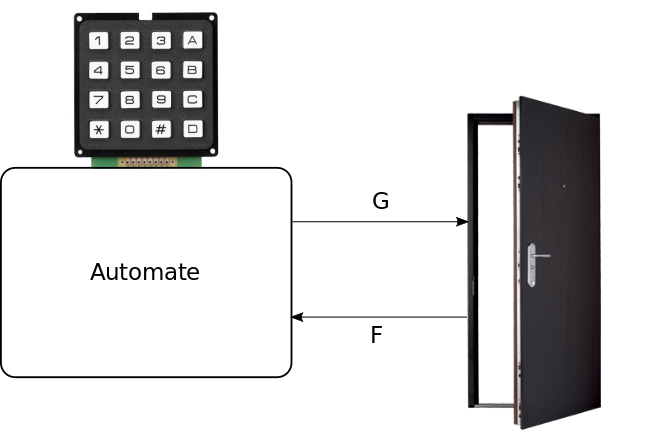
\includegraphics[scale=0.3]{./images/porte.png}
\caption{Schéma de principe de la a serrure numérique.}
\label{porte}
\end{figure}

Un capteur permet de connaître l'état de la porte : $F$ indique son état. $F$ vaut 1 si la porte est Fermée, et 0 si elle est ouverte.\\
$G$ commande l'ouverture de la porte : si $G=1$ la porte peut être ouverte. Lorsque la porte se referme, on a $G=0$.\\
À l'initialisation, la porte est fermée, le contact de porte $F=1$.\\
On précise qu'on ne peut appuyer que sur un seul bouton à la fois.

\begin{enumerate}
    \item Proposer un automate de contrôle du dispositif.
    \item Discuter de la robustesse de la solution, et de son réalisme. Proposer des alternatives.
    \item Optionnel : construire le circuit complet.
\end{enumerate}

\ifsolutions
\begin{solbox}
Dans ce type de dispositifs, les \textit{spécifications} du dispositif sont ambiguës et sujettes à interprétations. Cela est une constante dans ce type de systèmes !
\begin{itemize}
    \item Par exemple, est-il réaliste de ne pas prendre en compte un temps limite d'attente entre deux actions d'appui sur un bouton ? On pourrait donc, dans un état donné, déclencher un \textit{autre automate} dédié au décomptage du temps (timer).
    \item Ce timer est-il à déclencher \textit{entre} deux appuis, ou dès qu'on commence la séquence ?
    \item De même, le sujet stipule que la porte \textit{peut être ouverte} : cela ne signifie pas que le retrait de la gâche entraîne forcément l'ouverture de la porte : on devra donc là aussi attendre une action de l'utilisateur, probablement sur la poignée de la porte.
    \item S'il y a une poignée d'un côté de la porte, peut-on supposer qu'un \textit{autre} utilisateur puisse ouvrir la porte, de manière inopinée pendant la tentative du premier utilisateur ? Etc.
\end{itemize}

Nous proposons ici une solution à peu près réaliste : dès que la lettre A est correctement entrée, un timer se déclenche. Si la porte est par ailleurs ouverte (de l'intérieur), le dispositif se remet à l'état d'attente initial.

\centering
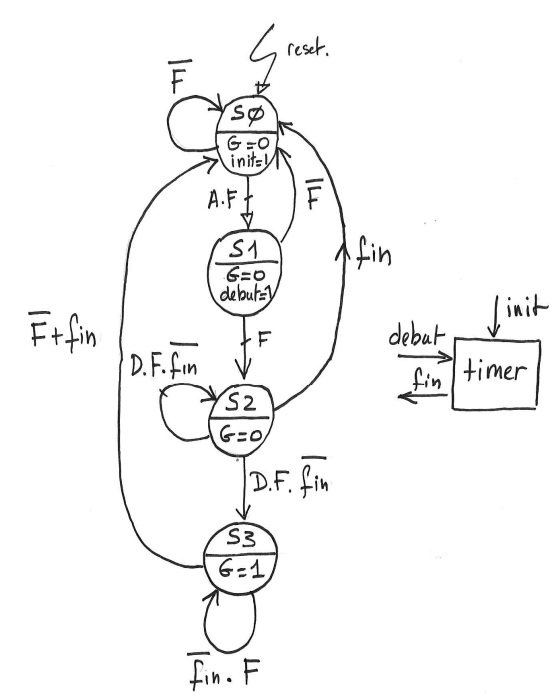
\includegraphics[scale=0.5]{./images/my_solution.png}
\captionof{figure}{Diagramme état-transition pour la serrure numérique. On fait appel à un autre dispositif numérique : un timer.}
\label{my_solution}
\end{solbox}
\fi
\end{document}
